\chapter{Literature Review}
\lhead{\emph{Literature Review}}
\label{LiteratureReview}
15-20 pages
\section{Processor Architectures for deep learning}

\subsection{High Performance Devices}
Include numbers here relating to memory and performance metrics from papers including speed, accuracy, model size
\subsubsection{GPUs}
Hardware structure, Benefits drawbacks and current performance on inference
\subsubsection{TPUs}
Structure, benefits, drawbacks, and current performance
\subsubsection{CPUs}
Hardware structure, drawbacks, current performance

\subsection{Low Power Edge Devices}
Numbers of memory and performance metrics for each of these
\subsubsection{FPGAs}
\begin{itemize}
\item
General Structure
\item
What makes them a good choice?
\end{itemize}

\subsubsection{USB Accelerators}
For each item in the list describe processor architecture and the current available performance figures
\begin{itemize}
\item
Intel Neural Compute Stick 
\begin{itemize}
\item
VPU Structure
\item
VPU Stats and figures
\end{itemize}
\item
Google Coral USB Accelerator
\begin{itemize}
\item
TPU At Edge

\end{itemize}
\end{itemize}

\subsubsection{Embedded GPUs}
Qualcomm Arduino line, Apple Bionic Chips.

Embedded within phones for example arm and apple
\subsubsection{Smart Home}
Google home now has neural processing units
\subsubsection{Edge Custom Solutions}
Current companies offering solutions focused on accelerating machine learning and neural network inference

Nvidia Jetson Line
NVIDIA EGX
Graphcore
Qualcomm
adapteva
viatech
mediatek - Supplimenting cloud ai chip in device NeuroPilot
Kalray
AWS Inferentia
Arm
Intel® Nervana™ Neural Network processors. Inside Xeon CPUs
custom asic

\section{Model Compression Techniques}
List of techniques and current results
\subsection{Methods/Algorithms}
\subsubsection{Pruning}
list of most interesting algorithms
how they work
Current available results
\subsubsection{Quantization}
Bit widths or weights and activation functions
\subsubsection{Knowledge Distillation}
\subsubsection{Regularization}
\subsubsection{Conditional Computation}

\subsection{Frameworks}
\begin{figure}
\centering
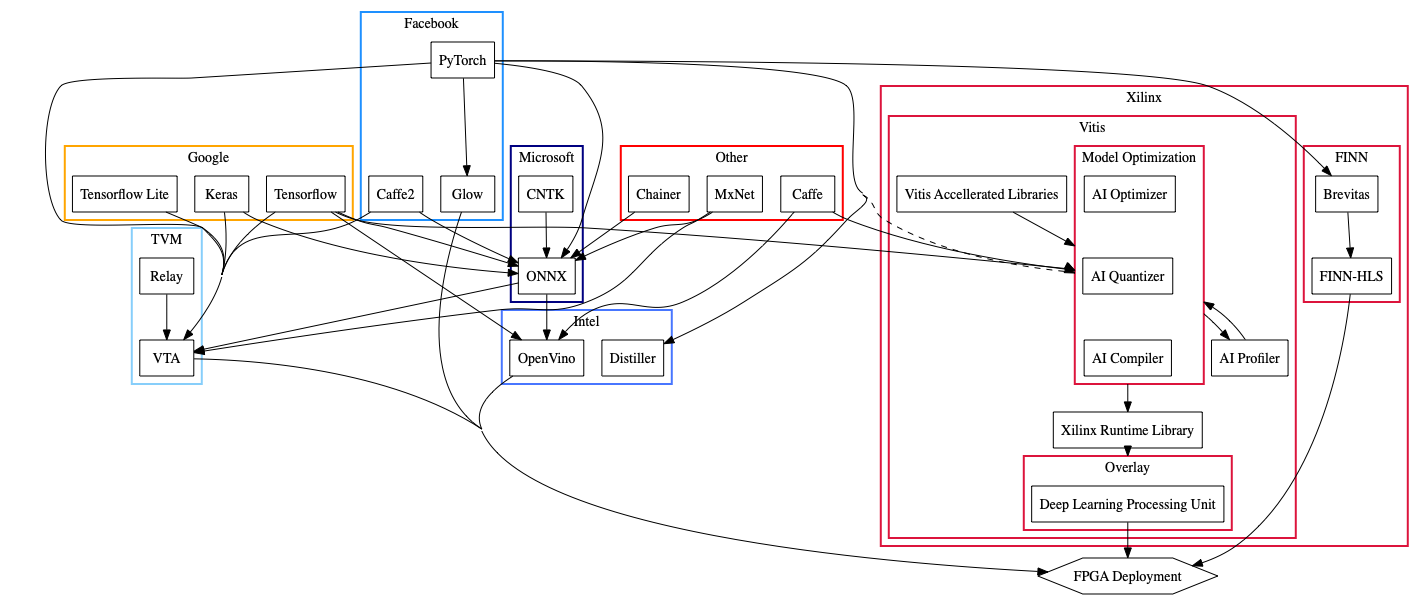
\includegraphics[width=\textwidth]{Figures/diagram.png}
\caption[Neural Network Frameworks]{The state of Neural Network Frameworks for Edge Deployment}
\label{fig:Neural Network Frameworks}
\end{figure}


\subsubsection{Intel Distiller}
\subsubsection{FINN}
\subsubsection{Intel OpenVino}
\subsubsection{Xilinx Vitis}

\section{Inference on edge devices}

\section{benchmarking Neural networks}

\subsection{Image classification}
\subsubsection{Datasets}
\subsection{Object Detection}
\subsubsection{Datasets}